\documentclass[runningheads,a4paper]{llncs}

\usepackage{verbatim}
\usepackage{amssymb}
\usepackage{amsmath} % Used for 'align' environment
\setcounter{tocdepth}{3}
\usepackage{graphicx} % Used for inserting pdf as graphics
\usepackage{float} % Used fo0r 'H' float option in figures
\usepackage{hyperref} % Used for creating a hyperlink to reference parts
\usepackage{enumitem}
\usepackage{textcomp}
\usepackage{multicol}
\usepackage{tikz}
\usetikzlibrary{positioning}
\usetikzlibrary{shapes.multipart}
\usetikzlibrary{shapes.misc} % used for rounded rectangle

\usepackage{multirow}
\usepackage{url}
\usepackage{color}
\urldef{\mailsa}\path|radelacruz@up.edu.ph|
\urldef{\mailsb}\path|fccabarle@up.edu.ph|
\urldef{\mailsc}\path|ivan.cedric10@gmail.com|
\urldef{\mailsd}\path|hnadorna@dcs.upd.edu.ph|
\urldef{\mailse}\path|zxxhust@gmail.com|
\usepackage{mathtools}
\DeclarePairedDelimiter\ceil{\lceil}{\rceil}
\DeclarePairedDelimiter\floor{\lfloor}{\rfloor}
    
\newcommand{\keywords}[1]{\par\addvspace\baselineskip
\noindent\keywordname\enspace\ignorespaces#1}
%\newcommand{\tt}[1]{\texttt{#1}}



\begin{document}

\mainmatter

\title
{
On Homogeneous Spiking Neural P System Variants
}

\titlerunning
{
Homogeneous SNPSP Systems
}


\author
{
Ren Tristan A. de la Cruz$^1$
\and
Francis George C. Cabarle$^{1,2}$
\and
Iva Cedric H. Macababayao$^{1}$
\and
Henry N. Adorna$^1$ 
\and
Xiangxiang Zeng$^3$
}

\authorrunning {de la Cruz et al}


\institute
{
$^1$Algorithms and Complexity Laboratory \\
Department of Computer Science, University of the Philippines - Diliman\\
Diliman 1101, Quezon City, Philippines    \\
$^2$Shenzhen Research Institute of Xiamen University \\
Xiamen University, Shenzhen 518000, Guangdong, China.\\
$^3$ School of Information Science and Engineering\\
Hunan University 410082, Changsha, China \\
\mailsa , \mailsb, \mailsc, \mailsd, \mailse 
}

\newcommand{\ra}{\rightarrow}

\toctitle{Lecture Notes in Computer Science}
\tocauthor{Authors' Instructions}


\maketitle

% ================================================================================================= %

\begin{abstract}

(ABSTRACT)

\keywords{Membrane Computing, 
          Spiking Neural P Systems, 
          Homogeneous Neurons,
          Structural Plasticity}
\end{abstract}

% ================================================================================================= %

\section{Introduction}

% ================================================================================================= %


\section{Spiking Neural P System and Some Variants} \label{sec-snps}

% ================================================================================================= %


\section{Homogenization of Spiking Neural P Systems} \label{sec-homo}

A \emph{state transition diagram} will be used to represent the activities of a neuron. 
A \emph{state} is a set of spike counts. For example, the state $\{4,5\}$ represents spike counts 
$4$ and $5$, the state $\{0,2,4,8,...\}$ represents even spike counts, and the state
$\{15,20,25,30,35,...\}$ represents spike counts that are multiples of $5$ starting from $15$. 

If a neuron has $n$ spikes, the neuron is said to be \emph{in state $S$} if $n \in S$. For example, 
let $n=10$ be the number spikes in the neuron and $S_a=\{1\}$, $S_b=\{2,4,9,10,...\}$, 
$S_c=\{5,10,15,20,...\}$ be states, the neuron is not in state $S_a$ since $n \notin S_a$ but it is
in state $S_b$ and $S_c$ since $n \in S_a$ and $n \in S_b$. States can intersect since they are 
sets which means a neuron can be in multiple states at the same time. 

Most states that are associated with a given neuron represent the regular expressions of the rules
in the neuron. For example, in Figure \ref{fig-two-neurons}, neuron $1$ have the rules
$r_1: a/a \ra \lambda$ and  $r_2: a^3(a^2)^*/a^2 \ra a$. The state $S_a=\{1\}$ represents the
regular expression $a$ of rule $r_1$ while the state $S_b=\{3,5,7,9,11,...\}$ represents the regular 
expression $a^3(a^2)^*$ of rule $r_2$. The state $S_c = \{0,2,4,6,8,...\}$, the set of even spike
counts, is also associated with neuron $1$ even though it does not represent a regular expression of
any of the rules in neuron $1$. State $S_c$ is relevant to neuron $1$ because neuron $1$ can be in
state $S_c$. For example, if neuron $1$ starts with $0$ spike and only receives even number of
spikes, then neuron $1$ will stay in state $S_3$.

For neuron $2$ in Figure \ref{fig-two-neurons}, it has the single rule $r_3: a^3/a^3 \ra a$ which 
means $S_z = \{3\}$ is associated with the neuron and it represents the regular expression $a^3$ of 
rule $r_3$. Neuron $2$ only has one incoming synapse so it can only receive one spike at a time 
assuming the use of non-extended/standard spiking rules. The only other relevant states for neuron 
$2$ are $S_w=\{0\}$, $S_x=\{1\}$, $s_y=\{2\}$. If neuron $2$ starts with $0$ spike, it will be state 
$S_w$. Neuron $2$ will be in state $S_x$ after receiving a spike, in state $S_y$ after receiving a 
total of $2$ spikes, and in state $S_z$ after receiving a total of $3$ spikes. At state $S_z$, 
neuron $2$ will use rule $r_3$ consuming $3$ spikes and  returning to state $S_w$. Only states
$S_w, S_x, S_y, S_z$ are relevant to neuron $2$ since it can only reach the spike counts in those
states.

\begin{figure}[H]                                                                                    
\begin{center}                                                                                         
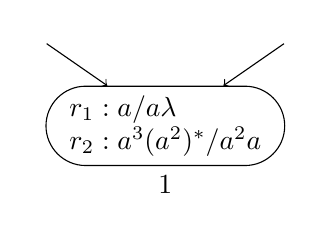
\begin{tikzpicture}                                                                                     
[                                                                                                       
neuron/.style={rounded rectangle, draw, minimum size = 10mm, align=left},                                                      
text-a/.style={black},                                                                                   
]                                                                                                       
\node (n1)   [neuron]                              {$r_1: a/a \ra \lambda$ \\ 
                                                    $r_2: a^3(a^2)^*/a^2 \ra a$};
\node (n1-d) [text-a, below       = 00.00mm of n1] {$1$};                                      
\node (s11)  [text-a, above right = 07.00mm of n1] {};                                      
\node (s12)  [text-a, above left  = 07.00mm of n1] {};
\draw [->]   (s11) -- (n1);                                    
\draw [->]   (s12) -- (n1);                                    
\end{tikzpicture}                                                                                       
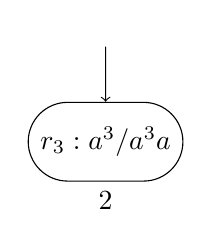
\begin{tikzpicture}                                                                                     
[                                                                                                       
neuron/.style={rounded rectangle, draw, minimum size = 10mm, align=left},                                                      
text-a/.style={black},                                                                                   
]                                                                                                       
\node (n2)   [neuron]                        {$r_3: a^3/a^3 \ra a$};
\node (n2-d) [text-a, below = 00.00mm of n2] {$2$};                                      
\node (s21)  [text-a, above = 07.00mm of n2] {};                                      
\draw [->]   (s21) -- (n2);                                    
\end{tikzpicture}                                                                                       
\end{center}
\caption{Example Neurons}                                                                                            
\label{fig-two-neurons}
\end{figure}                                                                                            

\begin{figure}[H]                                                                                    
\begin{center}                                                                                         
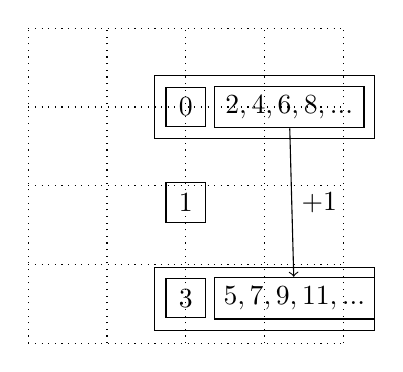
\begin{tikzpicture}
[
state/.style={rectangle, draw, minimum size = 5mm, align=left},                                                      
text-a/.style={black},                                                                                   
]
\draw [dotted] (-3,-3) grid (1,1);
\node (sc)  [state, minimum height = 08.00mm, minimum width = 28mm] at (0,0) {$ $};
\node (sc1) [state] at (-10mm,0) {$0$} ;
\node (sc2) [state, right = 01.00mm of sc1, minimum width = 19mm] {$2,4,6,8,...$}; 
\node (sa) [state, below = 07.00mm of sc1] {$1$};
\node (sb1) [state, below = 07.00mm of sa] {$3$};
\node (sb2) [state, right = 01.00mm of sb1] {$5,7,9,11,...$}; 
\node (sb)  [state, minimum height = 08.00mm, minimum width = 28mm] at (0,-2.44) {$ $};
\path [->] (sc2) edge node [right] {$+1$} (sb2);
\end{tikzpicture}

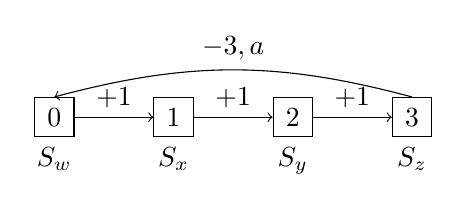
\begin{tikzpicture}                                                                                     
[                                                                                                       
state/.style={rectangle, draw, minimum size = 5mm, align=left},                                                      
text-a/.style={black},                                                                                   
]                                                                                                       
\node (sw)   [state]                              {$0$};
\node (swl)  [text-a, below = 00.00mm of sw]      {$S_w$};
\node (sx)   [state, right = 10.00mm of sw]       {$1$}; 
\node (sxl)  [text-a, below = 00.00mm of sx]      {$S_x$};
\node (sy)   [state, right = 10.00mm of sx]       {$2$}; 
\node (syl)  [text-a, below = 00.00mm of sy]      {$S_y$};
\node (sz)   [state, right = 10.00mm of sy]       {$3$}; 
\node (szl)  [text-a, below = 00.00mm of sz]      {$S_z$};
\draw [->]   (sw) edge node [above] {$+1$} (sx);                                    
\draw [->]   (sx) edge node [above] {$+1$} (sy);                                    
\draw [->]   (sy) edge node [above] {$+1$} (sz);                                    
%\draw [->]   (sz.north) edge [bend right=10] node [auto, swap] {$-3,a$} (sw.north);                                    
\path [->]   (sz.north) edge [bend right=15] node[above] {$-3,a$} (sw.north);                                    
%\draw  [->, bend above]   (sz.north) --  (sw.north);                                    
\end{tikzpicture}                                                                                       
\end{center}
\caption{Example Neurons}                                                                                            
\label{fig-two-state-diagrams}
\end{figure}                                                                                            

% ================================================================================================================================================== %

\bibliographystyle{splncs03}
\bibliography{homonegenous-snp}

\end{document}
